\FChapter{Chapter Nineteen}{19}

\Lettrine{T}{he} \textsc{library} looked tranquil enough as I entered it, and the Sibyl---if
Sibyl she were---was seated snugly enough in an easy-chair at the
chimney-corner. She had on a red cloak and a black bonnet: or rather, a
broad-brimmed gipsy hat, tied down with a striped handkerchief under her
chin. An extinguished candle stood on the table; she was bending over
the fire, and seemed reading in a little black book, like a prayer-book,
by the light of the blaze: she muttered the words to herself, as most
old women do, while she read; she did not desist immediately on my
entrance: it appeared she wished to finish a paragraph.

I stood on the rug and warmed my hands, which were rather cold with
sitting at a distance from the drawing-room fire. I felt now as
composed as ever I did in my life: there was nothing indeed in the
gipsy's appearance to trouble one's calm. She shut her book and slowly
looked up; her hat-brim partially shaded her face, yet I could see, as
she raised it, that it was a strange one. It looked all brown and
black: elf-locks bristled out from beneath a white band which passed
under her chin, and came half over her cheeks, or rather jaws: her eye
confronted me at once, with a bold and direct gaze.

\enquote{Well, and you want your fortune told?} she said, in a voice as
decided as her glance, as harsh as her features.

\enquote{I don't care about it, mother; you may please yourself: but I
	ought to warn you, I have no faith.}

\enquote{It's like your impudence to say so: I expected it of you; I
	heard it in your step as you crossed the threshold.}

\enquote{Did you? You've a quick ear.}

\enquote{I have; and a quick eye and a quick brain.}

\enquote{You need them all in your trade.}

\enquote{I do; especially when I've customers like you to deal with.
	Why don't you tremble?}

\enquote{I'm not cold.}

\enquote{Why don't you turn pale?}

\enquote{I am not sick.}

\enquote{Why don't you consult my art?}

\enquote{I'm not silly.}

The old crone \enquote{nichered} a laugh under her bonnet and bandage;
she then drew out a short black pipe, and lighting it began to smoke.
Having indulged a while in this sedative, she raised her bent body, took
the pipe from her lips, and while gazing steadily at the fire, said very
deliberately---\enquote{You are cold; you are sick; and you are silly.}

\enquote{Prove it,} I rejoined.

\enquote{I will, in few words. You are cold, because you are alone: no
	contact strikes the fire from you that is in you. You are sick; because
	the best of feelings, the highest and the sweetest given to man, keeps
	far away from you. You are silly, because, suffer as you may, you will
	not beckon it to approach, nor will you stir one step to meet it where
	it waits you.}

She again put her short black pipe to her lips, and renewed her smoking
with vigour.

\enquote{You might say all that to almost any one who you knew lived as
	a solitary dependent in a great house.}

\enquote{I might say it to almost any one: but would it be true of
	almost any one?}

\enquote{In my circumstances.}

\enquote{Yes; just so, in \emph{your} circumstances: but find me another
	precisely placed as you are.}

\enquote{It would be easy to find you thousands.}

\enquote{You could scarcely find me one. If you knew it, you are
	peculiarly situated: very near happiness; yes, within reach of it. The
	materials are all prepared; there only wants a movement to combine
	them. Chance laid them somewhat apart; let them be once approached and
	bliss results.}

\enquote{I don't understand enigmas. I never could guess a riddle in my
	life.}

\enquote{If you wish me to speak more plainly, show me your palm.}

\enquote{And I must cross it with silver, I suppose?}

\enquote{To be sure.}

I gave her a shilling: she put it into an old stocking-foot which she
took out of her pocket, and having tied it round and returned it, she
told me to hold out my hand. I did. She approached her face to the
palm, and pored over it without touching it.

\enquote{It is too fine,} said she. \enquote{I can make nothing of such
	a hand as that; almost without lines: besides, what is in a palm?
	Destiny is not written there.}

\enquote{I believe you,} said I\@.

\enquote{No,} she continued, \enquote{it is in the face: on the
	forehead, about the eyes, in the lines of the mouth. Kneel, and lift up
	your head.}

\enquote{Ah! now you are coming to reality,} I said, as I obeyed her.
\enquote{I shall begin to put some faith in you presently.}

I knelt within half a yard of her. She stirred the fire, so that a
ripple of light broke from the disturbed coal: the glare, however, as
she sat, only threw her face into deeper shadow: mine, it illumined.

\enquote{I wonder with what feelings you came to me to-night,} she said,
when she had examined me a while. \enquote{I wonder what thoughts are
	busy in your heart during all the hours you sit in yonder room with the
	fine people flitting before you like shapes in a magic-lantern: just as
	little sympathetic communion passing between you and them as if they
	were really mere shadows of human forms, and not the actual substance.}

\enquote{I feel tired often, sleepy sometimes, but seldom sad.}

\enquote{Then you have some secret hope to buoy you up and please you
	with whispers of the future?}

\enquote{Not I\@. The utmost I hope is, to save money enough out of my
	earnings to set up a school some day in a little house rented by
	myself.}

\enquote{A mean nutriment for the spirit to exist on: and sitting in
	that window-seat (you see I know your habits )---}

\enquote{You have learned them from the servants.}

\enquote{Ah! you think yourself sharp. Well, perhaps I have: to speak
	truth, I have an acquaintance with one of them, \Mrs{} Poole---}

I started to my feet when I heard the name.

\enquote{You have---have you?} thought I; \enquote{there is diablerie in
	the business after all, then!}

\enquote{Don't be alarmed,} continued the strange being; \enquote{she's
	a safe hand is \Mrs{} Poole: close and quiet; any one may repose
	confidence in her. But, as I was saying: sitting in that window-seat,
	do you think of nothing but your future school? Have you no present
	interest in any of the company who occupy the sofas and chairs before
	you? Is there not one face you study? one figure whose movements you
	follow with at least curiosity?}

\enquote{I like to observe all the faces and all the figures.}

\enquote{But do you never single one from the rest---or it may be, two?}

\enquote{I do frequently; when the gestures or looks of a pair seem
	telling a tale: it amuses me to watch them.}

\enquote{What tale do you like best to hear?}

\enquote{Oh, I have not much choice! They generally run on the same
	theme---courtship; and promise to end in the same
	catastrophe---marriage.}

\enquote{And do you like that monotonous theme?}

\enquote{Positively, I don't care about it: it is nothing to me.}

\enquote{Nothing to you? When a lady, young and full of life and
	health, charming with beauty and endowed with the gifts of rank and
	fortune, sits and smiles in the eyes of a gentleman you---}

\enquote{I what?}

\enquote{You know---and perhaps think well of.}

\enquote{I don't know the gentlemen here. I have scarcely interchanged
	a syllable with one of them; and as to thinking well of them, I consider
	some respectable, and stately, and middle-aged, and others young,
	dashing, handsome, and lively: but certainly they are all at liberty to
	be the recipients of whose smiles they please, without my feeling
	disposed to consider the transaction of any moment to me.}

\enquote{You don't know the gentlemen here? You have not exchanged a
	syllable with one of them? Will you say that of the master of the
	house!}

\enquote{He is not at home.}

\enquote{A profound remark! A most ingenious quibble! He went to
	Millcote this morning, and will be back here to-night or to-morrow: does
	that circumstance exclude him from the list of your acquaintance---blot
	him, as it were, out of existence?}

\enquote{No; but I can scarcely see what \Mr{} Rochester has to do with
	the theme you had introduced.}

\enquote{I was talking of ladies smiling in the eyes of gentlemen; and
	of late so many smiles have been shed into \Mr{} Rochester's eyes that
	they overflow like two cups filled above the brim: have you never
	remarked that?}

\enquote{\Mr{} Rochester has a right to enjoy the society of his guests.}

\enquote{No question about his right: but have you never observed that,
	of all the tales told here about matrimony, \Mr{} Rochester has been
	favoured with the most lively and the most continuous?}

\enquote{The eagerness of a listener quickens the tongue of a
	narrator.} I said this rather to myself than to the gipsy, whose
strange talk, voice, manner, had by this time wrapped me in a kind of
dream. One unexpected sentence came from her lips after another, till I
got involved in a web of mystification; and wondered what unseen spirit
had been sitting for weeks by my heart watching its workings and taking
record of every pulse.

\enquote{Eagerness of a listener!} repeated she: \enquote{yes; \Mr{}
	Rochester has sat by the hour, his ear inclined to the fascinating lips
	that took such delight in their task of communicating; and \Mr{} Rochester
	was so willing to receive and looked so grateful for the pastime given
	him; you have noticed this?}

\enquote{Grateful! I cannot remember detecting gratitude in his face.}

\enquote{Detecting! You have analysed, then. And what did you detect,
	if not gratitude?}

I said nothing.

\enquote{You have seen love: have you not?---and, looking forward, you
	have seen him married, and beheld his bride happy?}

\enquote{Humph! Not exactly. Your witch's skill is rather at fault
	sometimes.}

\enquote{What the devil have you seen, then?}

\enquote{Never mind: I came here to inquire, not to confess. Is it
	known that \Mr{} Rochester is to be married?}

\enquote{Yes; and to the beautiful Miss Ingram.}

\enquote{Shortly?}

\enquote{Appearances would warrant that conclusion: and, no doubt
	(though, with an audacity that wants chastising out of you, you seem to
	question it), they will be a superlatively happy pair. He must love
	such a handsome, noble, witty, accomplished lady; and probably she loves
	him, or, if not his person, at least his purse. I know she considers
	the Rochester estate eligible to the last degree; though (God pardon
	me!) I told her something on that point about an hour ago which made her
	look wondrous grave: the corners of her mouth fell half an inch. I
	would advise her blackaviced suitor to look out: if another comes, with
	a longer or clearer rent-roll,---he's dished---}

\enquote{But, mother, I did not come to hear \Mr{} Rochester's fortune: I
	came to hear my own; and you have told me nothing of it.}

\enquote{Your fortune is yet doubtful: when I examined your face, one
	trait contradicted another. Chance has meted you a measure of
	happiness: that I know. I knew it before I came here this evening. She
	has laid it carefully on one side for you. I saw her do it. It depends
	on yourself to stretch out your hand, and take it up: but whether you
	will do so, is the problem I study. Kneel again on the rug.}

\enquote{Don't keep me long; the fire scorches me.}

\begin{figure}
	\begin{sidecaption}{She did not stoop towards me,\linebreak but only gazed,\linebreak leaning back in her chair.}[p190b]
		\centering
		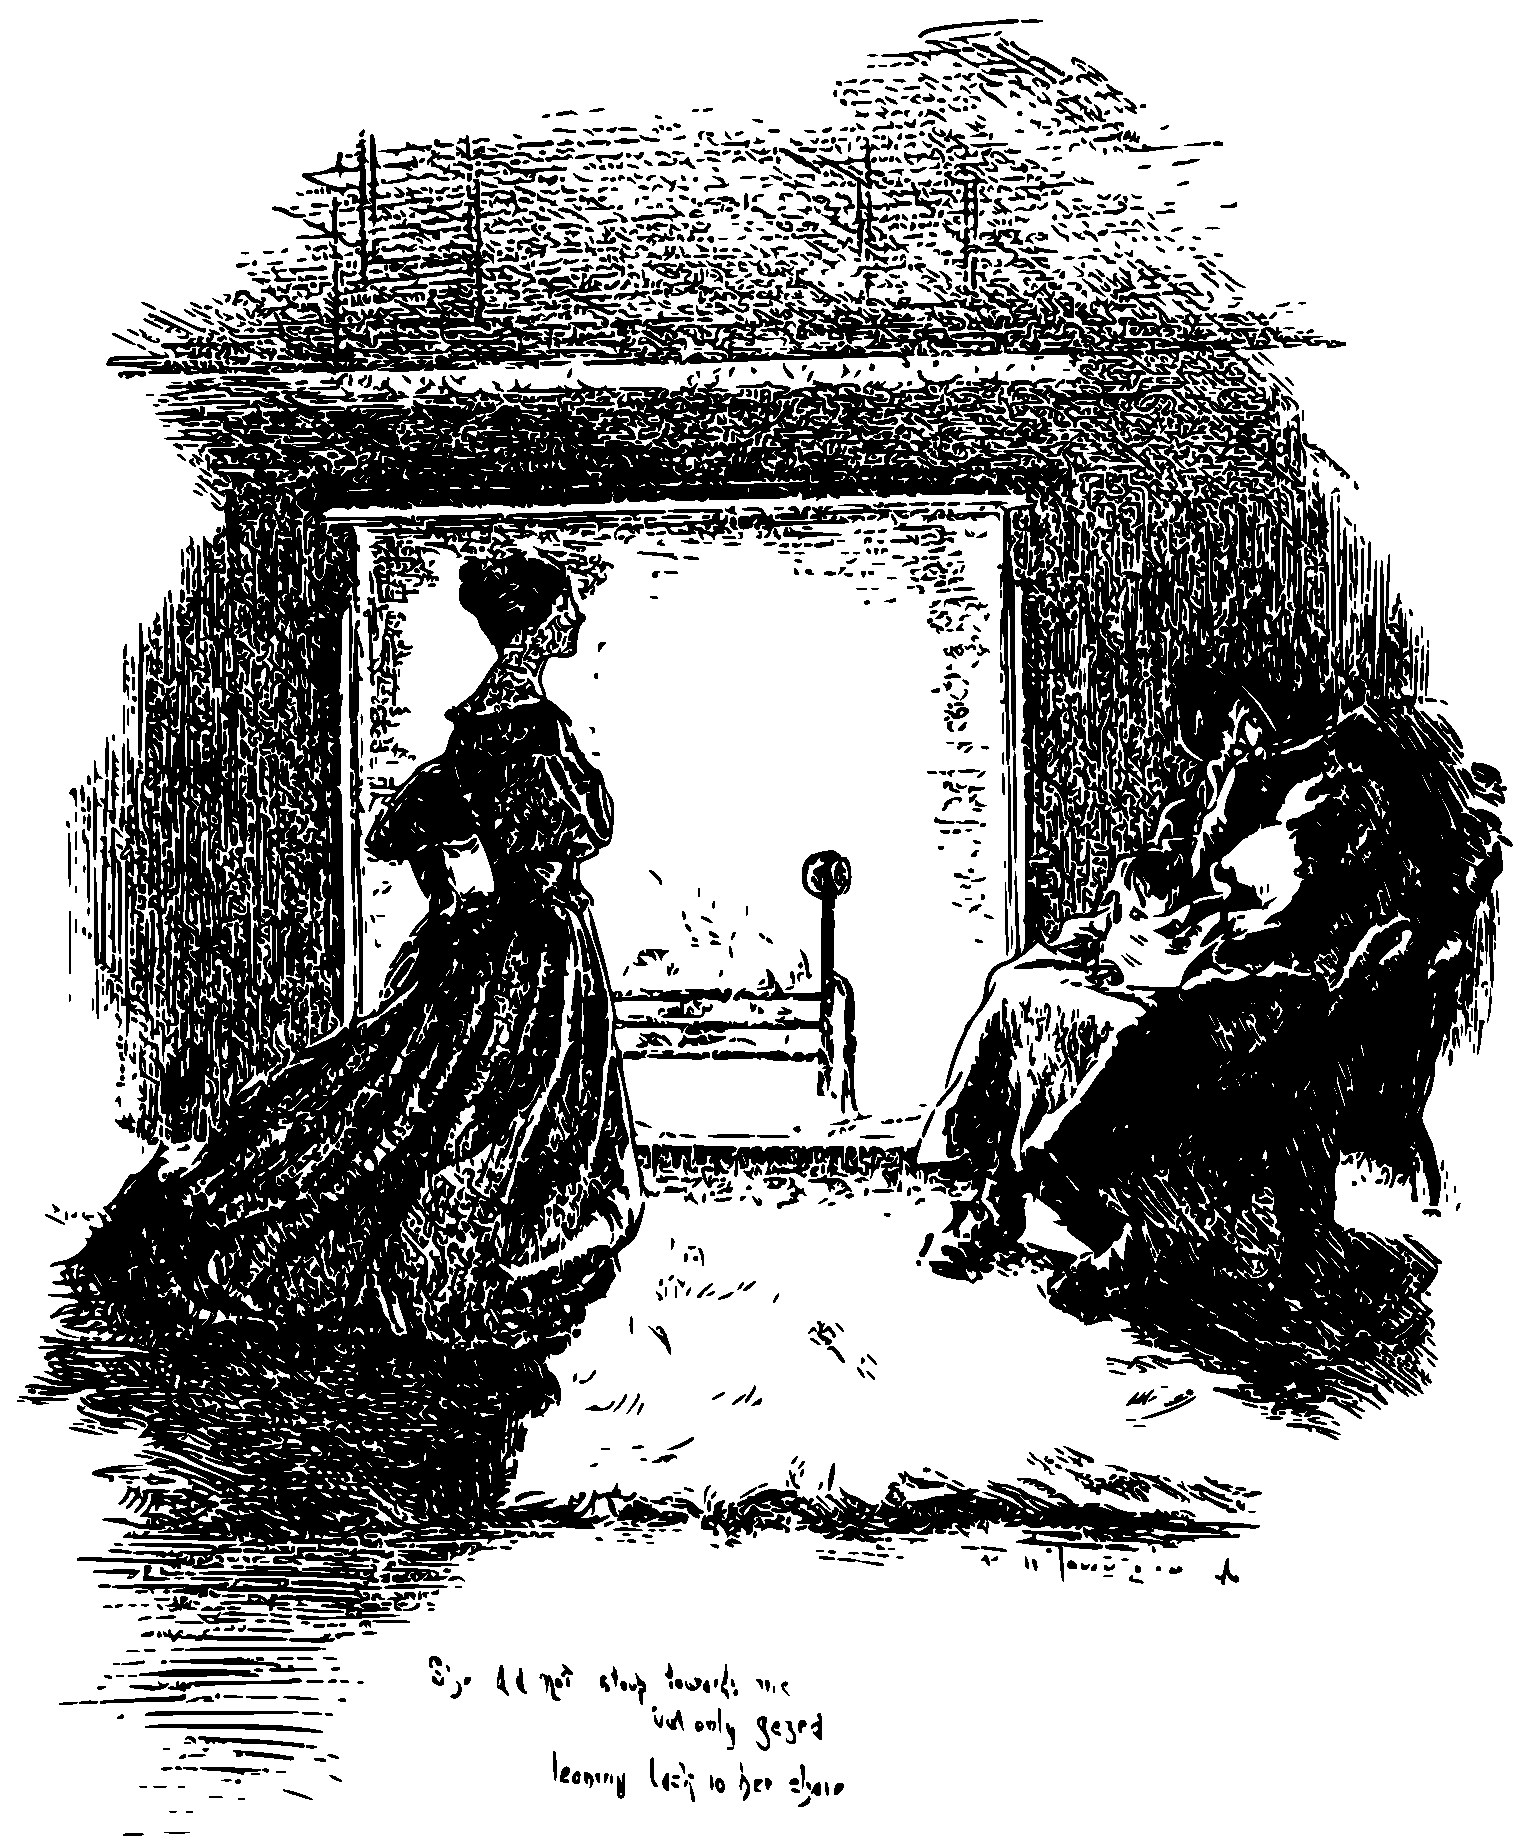
\includegraphics[width=\linewidth]{images/p190b.pdf}
	\end{sidecaption}
\end{figure}

I knelt. She did not stoop towards me, but only gazed, leaning back in
her chair. She began muttering,---

\enquote{The flame flickers in the eye; the eye shines like dew; it looks soft
	and full of feeling; it smiles at my jargon: it is susceptible;
	impression follows impression through its clear sphere; where it ceases
	to smile, it is sad; an unconscious lassitude weighs on the lid: that
	signifies melancholy resulting from loneliness. It turns from me; it
	will not suffer further scrutiny; it seems to deny, by a mocking glance,
	the truth of the discoveries I have already made,---to disown the charge
	both of sensibility and chagrin: its pride and reserve only confirm me
	in my opinion. The eye is favourable.

	%rem enq
	As to the mouth, it delights at times in laughter; it is disposed to
	impart all that the brain conceives; though I daresay it would be silent
	on much the heart experiences. Mobile and flexible, it was never
	intended to be compressed in the eternal silence of solitude: it is a
	mouth which should speak much and smile often, and have human affection
	for its interlocutor. That feature too is propitious.

	%rem enq
	I see no enemy to a fortunate issue but in the brow; and that brow
	professes to say,---\enquote{I can live alone, if self-respect, and
		circumstances require me so to do. I need not sell my soul to buy
		bliss. I have an inward treasure born with me, which can keep me alive
		if all extraneous delights should be withheld, or offered only at a
		price I cannot afford to give.} The forehead declares, \enquote{Reason
		sits firm and holds the reins, and she will not let the feelings burst
		away and hurry her to wild chasms. The passions may rage furiously,
		like true heathens, as they are; and the desires may imagine all sorts
		of vain things: but judgment shall still have the last word in every
		argument, and the casting vote in every decision. Strong wind,
		earthquake-shock, and fire may pass by: but I shall follow the guiding
		of that still small voice which interprets the dictates of conscience.}

	%rem enq
	Well said, forehead; your declaration shall be respected. I have
	formed my plans---right plans I deem them---and in them I have attended
	to the claims of conscience, the counsels of reason. I know how soon
	youth would fade and bloom perish, if, in the cup of bliss offered, but
	one dreg of shame, or one flavour of remorse were detected; and I do not
	want sacrifice, sorrow, dissolution---such is not my taste. I wish to
	foster, not to blight---to earn gratitude, not to wring tears of
	blood---no, nor of brine: my harvest must be in smiles, in endearments,
	in sweet---That will do. I think I rave in a kind of exquisite
	delirium. I should wish now to protract this moment \emph{ad
		infinitum}; but I dare not. So far I have governed myself thoroughly.
	I have acted as I inwardly swore I would act; but further might try me
	beyond my strength. Rise, Miss Eyre: leave me; the play is played
	out'.}

Where was I? Did I wake or sleep? Had I been dreaming? Did I dream
still? The old woman's voice had changed: her accent, her gesture, and
all were familiar to me as my own face in a glass---as the speech of my
own tongue. I got up, but did not go. I looked; I stirred the fire,
and I looked again: but she drew her bonnet and her bandage closer about
her face, and again beckoned me to depart. The flame illuminated her
hand stretched out: roused now, and on the alert for discoveries, I at
once noticed that hand. It was no more the withered limb of eld than my
own; it was a rounded supple member, with smooth fingers, symmetrically
turned; a broad ring flashed on the little finger, and stooping forward,
I looked at it, and saw a gem I had seen a hundred times before. Again
I looked at the face; which was no longer turned from me---on the
contrary, the bonnet was doffed, the bandage displaced, the head
advanced.

\enquote{Well, Jane, do you know me?} asked the familiar voice.

\enquote{Only take off the red cloak, sir, and then---}

\enquote{But the string is in a knot---help me.}

\enquote{Break it, sir.}

\enquote{There, then---\enquote{Off, ye lendings!}} And \Mr{} Rochester stepped
out of his disguise.

\enquote{Now, sir, what a strange idea!}

\enquote{But well carried out, eh? Don't you think so?}

\enquote{With the ladies you must have managed well.}

\enquote{But not with you?}

\enquote{You did not act the character of a gipsy with me.}

\enquote{What character did I act? My own?}

\enquote{No; some unaccountable one. In short, I believe you have been
	trying to draw me out---or in; you have been talking nonsense to make me
	talk nonsense. It is scarcely fair, sir.}

\enquote{Do you forgive me, Jane?}

\enquote{I cannot tell till I have thought it all over. If, on
	reflection, I find I have fallen into no great absurdity, I shall try to
	forgive you; but it was not right.}

\enquote{Oh, you have been very correct---very careful, very sensible.}

I reflected, and thought, on the whole, I had. It was a comfort; but,
indeed, I had been on my guard almost from the beginning of the
interview. Something of masquerade I suspected. I knew gipsies and
fortune-tellers did not express themselves as this seeming old woman had
expressed herself; besides I had noted her feigned voice, her anxiety to
conceal her features. But my mind had been running on Grace
Poole---that living enigma, that mystery of mysteries, as I considered
her. I had never thought of \Mr{} Rochester.

\enquote{Well,} said he, \enquote{what are you musing about? What does
	that grave smile signify?}

\enquote{Wonder and self-congratulation, sir. I have your permission to
	retire now, I suppose?}

\enquote{No; stay a moment; and tell me what the people in the
	drawing-room yonder are doing.}

\enquote{Discussing the gipsy, I daresay.}

\enquote{Sit down!---Let me hear what they said about me.}

\enquote{I had better not stay long, sir; it must be near eleven
	o'clock. Oh, are you aware, \Mr{} Rochester, that a stranger has arrived
	here since you left this morning?}

\enquote{A stranger!---no; who can it be? I expected no one; is he
	gone?}

\enquote{No; he said he had known you long, and that he could take the
	liberty of installing himself here till you returned.}

\enquote{The devil he did! Did he give his name?}

\enquote{His name is Mason, sir; and he comes from the West Indies; from
	Spanish Town, in Jamaica, I think.}

\Mr{} Rochester was standing near me; he had taken my hand, as if to lead
me to a chair. As I spoke he gave my wrist a convulsive grip; the smile
on his lips froze: apparently a spasm caught his breath.

\enquote{Mason!---the West Indies!} he said, in the tone one might fancy
a speaking automaton to enounce its single words; \enquote{Mason!---the
	West Indies!} he reiterated; and he went over the syllables three times,
growing, in the intervals of speaking, whiter than ashes: he hardly
seemed to know what he was doing.

\enquote{Do you feel ill, sir?} I inquired.

\enquote{Jane, I've got a blow; I've got a blow, Jane!} He staggered.

\enquote{Oh, lean on me, sir.}

\enquote{Jane, you offered me your shoulder once before; let me have it
	now.}

\enquote{Yes, sir, yes; and my arm.}

He sat down, and made me sit beside him. Holding my hand in both his
own, he chafed it; gazing on me, at the same time, with the most
troubled and dreary look.

\enquote{My little friend!} said he, \enquote{I wish I were in a quiet
	island with only you; and trouble, and danger, and hideous recollections
	removed from me.}

\enquote{Can I help you, sir?---I'd give my life to serve you.}

\enquote{Jane, if aid is wanted, I'll seek it at your hands; I promise
	you that.}

\enquote{Thank you, sir. Tell me what to do,---I'll try, at least, to
	do it.}

\enquote{Fetch me now, Jane, a glass of wine from the dining-room: they
	will be at supper there; and tell me if Mason is with them, and what he
	is doing.}

I went. I found all the party in the dining-room at supper, as \Mr{}
Rochester had said; they were not seated at table,---the supper was
arranged on the sideboard; each had taken what he chose, and they stood
about here and there in groups, their plates and glasses in their
hands. Every one seemed in high glee; laughter and conversation were
general and animated. \Mr{} Mason stood near the fire, talking to Colonel
and \Mrs{} Dent, and appeared as merry as any of them. I filled a
wine-glass (I saw Miss Ingram watch me frowningly as I did so: she
thought I was taking a liberty, I daresay), and I returned to the
library.

\Mr{} Rochester's extreme pallor had disappeared, and he looked once more
firm and stern. He took the glass from my hand.

\enquote{Here is to your health, ministrant spirit!} he said. He
swallowed the contents and returned it to me. \enquote{What are they
	doing, Jane?}

\enquote{Laughing and talking, sir.}

\enquote{They don't look grave and mysterious, as if they had heard
	something strange?}

\enquote{Not at all: they are full of jests and gaiety.}

\enquote{And Mason?}

\enquote{He was laughing too.}

\enquote{If all these people came in a body and spat at me, what would
	you do, Jane?}

\enquote{Turn them out of the room, sir, if I could.}

He half smiled. \enquote{But if I were to go to them, and they only
	looked at me coldly, and whispered sneeringly amongst each other, and
	then dropped off and left me one by one, what then? Would you go with
	them?}

\enquote{I rather think not, sir: I should have more pleasure in staying
	with you.}

\enquote{To comfort me?}

\enquote{Yes, sir, to comfort you, as well as I could.}

\enquote{And if they laid you under a ban for adhering to me?}

\enquote{I, probably, should know nothing about their ban; and if I did,
	I should care nothing about it.}

\enquote{Then, you could dare censure for my sake?}

\enquote{I could dare it for the sake of any friend who deserved my
	adherence; as you, I am sure, do.}

\enquote{Go back now into the room; step quietly up to Mason, and
	whisper in his ear that \Mr{} Rochester is come and wishes to see him:
	show him in here and then leave me.}

\enquote{Yes, sir.}

I did his behest. The company all stared at me as I passed straight
among them. I sought \Mr{} Mason, delivered the message, and preceded him
from the room: I ushered him into the library, and then I went upstairs.

At a late hour, after I had been in bed some time, I heard the visitors
repair to their chambers: I distinguished \Mr{} Rochester's voice, and
heard him say, \enquote{This way, Mason; this is your room.}

He spoke cheerfully: the gay tones set my heart at ease. I was soon
asleep.
